
\subsection{Laden vom Simulink Modell}

Damit wir mit dem Simulink Modell arbeiten können, muss dies zunächst in das Matlab Skript eingebunden werden. 
Hierfür wird die Simulink Funktion load\_model verwendet, um das Simulink Modell in den Matlab Arbeitsbereich zu laden. 
Anschließend können die Eingänge des Modells mit der Funktion set\_param angepasst werden, um die gewünschte Geschwindigkeit zu simulieren.
Die Simulation wird für verschiedene Geschwindigkeiten durchgeführt, und der stationäre Schwimmwinkel wird für jede Geschwindigkeit berechnet.
Somit können wir die Schwimmwinkelwerte für die verschiedenen Geschwindigkeiten vergleichen und die optimale Geschwindigkeit bestimmen, bei der der stationäre Schwimmwinkel minimal ist.

\subsection{stationäre Schwimmwinkel in eingeschwungenen Zustand}
Die Simulationsergebnisse liefern uns die Time Series Daten für den Schwimmwinkel über die Zeit. Um den stationären Schwimmwinkel $\beta_{ss} = \lim_{t \to \infty} \beta(t)$ im eingeschwungenen Zustand zu bestimmen, betrachten
wir den Mittelwert des Schwimmwinkels in der letzten Sekunde der Simulation. Dieser Mittelwert dient als Näherung für den stationären Schwimmwinkel, 
da sich das System in diesem Zeitraum bereits eingependelt hat und die transienten Effekte weitgehend abgeklungen sind.

Für die Optimierung der Geschwindigkeit simulieren wir das Einspurmodell für verschiedene Geschwindigkeiten und berechnen jeweils den stationären Schwimmwinkel, damit definieren wir eine Funktion 
$\beta_{ss}(v)$, die den stationären Schwimmwinkel in Abhängigkeit von der Geschwindigkeit $v$ angibt.

\subsection{Optimale Geschwindigkeit}
Die optimale Geschwindigkeit wird durch die Minimierung des Betrags des stationären Schwimmwinkels $\beta_{ss}(v)$ bestimmt. Hierfür verwenden wir die Funktion \emph{fminbnd}, die eine eindimensionale Funktion minimiert.
Die Funktion fminbnd benötigt als Eingabe eine Funktion, die in einem gegebenen Intervall minimiert werden soll. In unserem Fall ist die Funktion, die minimiert werden soll, der Betrag des stationären Schwimmwinkels $\beta_{ss}(v)^2$ 
und das Intervall für die Geschwindigkeit $v$ wird entsprechend der realistischen Fahrgeschwindigkeiten festgelegt, z.B. von 0 bis 200 km/h.

\newpage
\subsection{Güte Funktion}
Wie schon in vorherigen Abschnitt beschrieben, minimiert die Funktion \emph{fminbnd} den Betrag des stationären Schwimmwinkels. Das ist eine Art 
Nullstellenbestimmung, da wir die Geschwindigkeit suchen, bei der der stationäre Schwimmwinkel möglichst nahe bei Null liegt.

\begin{equation*}
    v_{opt} = \arg\min_{v} |\beta_{ss}(v)|
\end{equation*}

für 

\begin{equation*}
    \beta_{ss}(v) \rightarrow^{v \to v_{opt}} 0
\end{equation*}


Da fminbnd keine Nullstellen, sondern Minima auf einem Intervall bestimmt, wird das Problem in ein Minimierungsproblem überführt. Dazu definieren wir eine nichtnegative Zielfunktion, eine Gütefunktion $\phi(v)$
\begin{equation*}
    \phi(x) := g(x)^2
\end{equation*}

Dann gilt:
\begin{equation*}
    \phi(x) \geq 0 \quad \forall x
\end{equation*}
\begin{equation*}
    \phi(x) = 0 \Leftrightarrow g(x) = 0
\end{equation*}

Damit ist jede Nullstelle von $g$ eine globale Minimierungsstelle von $\phi$ mit Minimalwert 0.
Also kann man die Nullstellenbestimmung als
\begin{equation*}
    \arg\min_{x} \phi(x) = \arg\min_{x} g(x)^2
\end{equation*}
formulieren, was mit \emph{fminbnd} gelöst werden kann.

\newpage

\subsection{Optimale Geschwindigkeit und Interpretation des Fahrverhaltens}

Die Optimale Geschwindigkeit $v_{opt}$, bei der der stationäre Schwimmwinkel minimal ist, wurde durch die Anwendung der Funktion \emph{fminbnd} auf die Funktion $\beta_{ss}(v)^2$ bestimmt. 
mit: 
\begin{equation*}
    v_{opt} = 13,93 \mathrm{m/s} \approx 50,15 \mathrm{km/h}
\end{equation*}

und dem entsprechenden stationären Schwimmwinkel von:
\begin{equation*}
    \beta_{ss}(v_{opt}) \approx 0 
\end{equation*}

\begin{figure}[H]
    \centering
    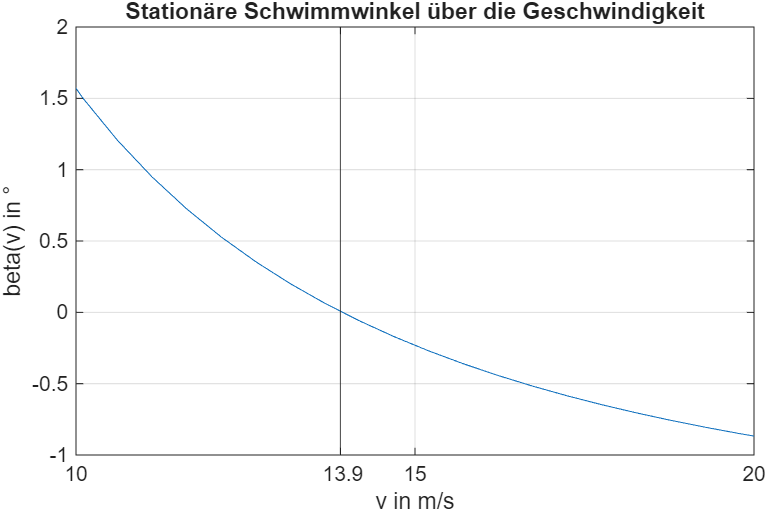
\includegraphics[width=0.75\linewidth]{pictures/ss_beta_ueber_v .png}
    \caption{Entwicklung des stationären Schwimmwinkels $\beta_{ss}$ über die Geschwindigkeit $v$.}
    \label{fig:schraeglaufwinkelVerlauf}

\end{figure}

Abbildung~\ref{fig:schraeglaufwinkelVerlauf} zeigt die Entwicklung des stationären Schwimmwinkels $\beta_{ss}$ über die Geschwindigkeit $v$ 
und dass bei der optimalen Geschwindigkeit von etwa 50 km/h der stationäre Schwimmwinkel nahezu null ist, was auf eine stabile Fahrdynamik hinweist,
bedeutet, dass der richtung der Fahrzeugbewegung $\delta$ bei der Geschwindigkeit mit der Fahrzeuglängsrichtung $v_s$ übereinstimmt. 
Bei niedereren Geschwindigkeiten hat der Schwimmwinkel einen positiven Wert, was darauf hindeutet, dass 
die Fahrzeugbewegung links von der Richtung der Fahrzeuglängsrichtung abweicht
und bei höheren Geschwindigkeiten hat der Schwimmwinkel einen negativen Wert, was darauf hindeutet, dass die Fahrzeugbewegung rechts von der Richtung der Fahrzeuglängsrichtung abweicht.


\begin{figure}[H]
    \centering
    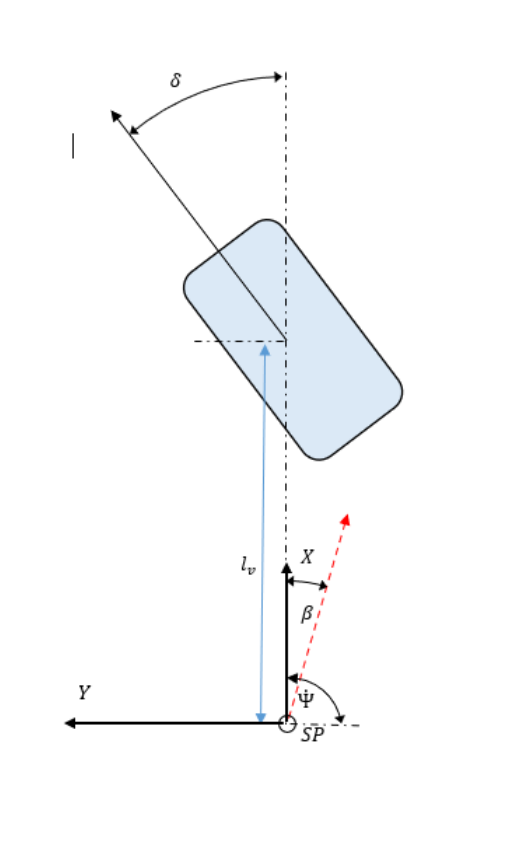
\includegraphics[width=0.5\linewidth]{pictures/schwimm.png}
    \caption{Darstellung des Schwimmwinkels im Einspurmodell.}
    \label{fig:schwimmmwinkel}

\end{figure}

Anmerkung: Der rote gestrichelte Pfeil in Abbildung~\ref{fig:schwimmmwinkel} zeigt die Richtung der Fahrzeugbewegung $v_s$, die durch den Schwimmwinkel $\beta$ von der Fahrzeuglängsrichtung $v$ abweicht.
